\documentclass{boi2014-dk}

\usepackage{enumitem}
\usepackage{wrapfig}
\usepackage{mathtools}
\usepackage{tikz}

\renewcommand{\DayNum}{1}
\renewcommand{\TaskCode}{coprobber}
\renewcommand{\TaskName}{The Cop and the Robber}
\renewcommand{\TaskVersion}{1.4}

\renewcommand{\labelitemii}{$\circ$}
\newcommand{\constant}[1]{{\tt #1}}

\begin{document}
    \begin{wrapfigure}[8]{r}{6cm}
        \vspace{-24pt}
		\includegraphics[width=6cm]{\TaskCode.jpeg}
	\end{wrapfigure}

	I byen, Bytemore, er kriminalitetsniveauet nået et nyt højdepunkt.
	Blandt andre ugerninger, sker der røverier hver eneste dag.
	Når en kriminel handling bliver begået, er det altid op til
	en enlig patruljerende politibetjent at jage røveren gennem
	smalle gader der forbinder gadehjørner (der ofte blot bliver
	benævnt \emph{hjørner}). Uheldigvis undslipper røverne som regel
	deres efterfølgere, fordi de kender byen meget bedre end politiet.

	Bytemore City Police Department (BCPD) organiserer et topmøde
	for at reducere kriminaliteten. Et af initiativerne er at bruge
	computerhjælp når røverne skal fanges. For at gøre dette har
	BCPD lavet et præcist kort over byen. Nu har de brug for et
	program til at finde jagtstrategier.

	Jagtproblemet, hvor én betjent jager en røver er modelleret på
	følgende måde:
    \begin{enumerate}
    	\item Politibetjenten vælger et hjørne at patruljere på.
    	\item Røveren vælger derefter et hjørne til røveriet
    		  (Han ved hvor betjenten er). Fra dette øjeblik
    		  er det hele tiden antaget at både betjenten og
    		  røveren ved hvor den anden er.
    	\item Politibetjentens træk består af at han flytter til
    		  et nabo-hjørne (dvs. et, der er forbundet til det
    		  nuværende af en gade) eller venter (dvs. undlader
    		  at flytte).
    	\item Røverens træk består af at han flytter sig til et
    		  nabo-hjørne. Bemærk, at røveren, ulig betjenten,
    		  ikke kan vente. Det ligger i hans natur at blive
    		  ved med at flygte.
    	\item Politibetjenten og røveren bliver ved med at skiftes
    		  til at lave et træk (startende med betjenten) indtil
    		  en af de følgende ting sker:
        \begin{enumerate}
        	\item Situationen gentager sig selv (situationen er
        		  defineret ved position af betjenten, samt røveren
        		  og hvis tur det er til at trække). Dette svarer
        		  til at røveren kan undgå politibetjenten for
        		  evigt, så røveren undslipper.
        	\item Politibetjenten og røveren mødes på det samme
        		  hjørne efter en af dem har lavet et træk. I dette
        		  tilfælde fanger politibetjenten røveren.
        \end{enumerate}
    \end{enumerate}

    \Task
    Du skal skrive et program, der givet et kort over byen, skal
    bestemme hvorvidt det er muligt at fange røveren, og, hvis det
    er, skal fange røveren ved at lave træk på vegne af
    politibetjenten.

	Dit program skal antage at røveren trækker optimalt.

    \Implementation
    Du skal implementere to funktioner:
    \begin{itemize}
        \item \method{start(N, A)} der tager følgende parametre:
            \begin{itemize}
                \item $N$ --- antallet af hjørner (hjørnerne er navngivet
                	  $0$ til $N-1$).
                \item $A$ --- et to-dimensionelt array der beskriver
                	  gaderne: for $0 \le i, j \le N-1$,
                      $$
                          A[i, j] \text{ is }
                          \begin{dcases*}
                              \texttt{false} & if $i$ and $j$ are not
                                               joined by any alley
                                \\
                              \texttt{true} & if $i$ and $j$ are joined
                                              by an alley
                          \end{dcases*}
                      $$
                      Man kan gå begge veje igennem alle gader (dvs.
                      $A[i, j] = A[j, i]$ for alle værdier af $i$ og $j$) og
                      dervil ikke være nogen gader der forbinder et hjørne til
                      sig selv (dvs. $A[i, i]$ vil være \texttt{false} for
                      alle værdier af $i$). Derudover må du antage at det altid
                      vil være muligt at nå ethvert hjørne fra ethvert andet
                      hjørne ved at gå igennem gaderne.
            \end{itemize}
            Hvis det er muligt at fange røveren på det beskrevne kort, skal
            funktionen \method{start} returnere navnet på det hjørne, som
            politibetjenten vælger at patruljere. Ellers skal $-1$
            returneres.

        \item \method{nextMove(R)} der som en parameter tager navnet $R$
		      på det hjørne som røveren står på nu og skal returnere
		      navnet på det hjørne, som betjenten vil være på efter sit
		      træk.
    \end{itemize}

	Funktionen \method{start} vil blive kaldt præcis én gang før
	noget kald til \method{nextMove} bliver lavet. Hvis
	\method{start} returnerer $-1$, så vil \method{nextMove} ikke
	blive kaldt. Ellers vil \method{nextMove} blive kaldt
	gentagne gange indtil forfølgelsen slutter. Mere præcist vil
	programmet afslutte så snart at en af de følgende ting sker:
    \begin{itemize}
        \item \method{nextMove} returnerer et ugyldigt træk.
        \item Situationen gentager sig selv.
        \item Røveren bliver fanget.
    \end{itemize}

    \Example
    \begin{wrapfigure}[4]{r}{2cm}
        \vspace{-0.5cm}
        \centering
        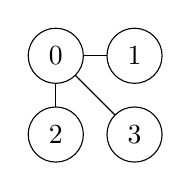
\begin{tikzpicture}
        \draw (0,1) -- (0,0);
        \draw (0,1) -- (1,0);
        \draw (0,1) -- (1,1);
        \foreach \x in {0,1} \foreach \y in {0,1}
            \draw (\x,\y) node[circle,draw,fill=white,inner sep=0,minimum size=0.7cm] {\pgfmathparse{int(2-2*\y+\x)}\pgfmathresult};
        \end{tikzpicture}
    \end{wrapfigure}
	Lad os kigge på eksemplet illustreret til højre. I dette tilfælde
	er ethvert hjørne en god startposition for politibetjenten. Hvis
	han starter i hjørnet 0, kan han vente i sit første træk og røveren
	vil løbe ind i ham. På den anden side, hvis han starter på et andet
	hjørne, kan han vente indtil røveren flytter sig til hjørne 0, og
	derefter flytte derhen.

    En kørsel kunne se således ud:

    \begin{tabular}{|l|c|}
        \hline
            {\bf Function call} & {\bf Returns} \\
        \hline
            \method{start(4, [[0, 1, 1, 1], [1, 0, 0, 0], [1, 0, 0, 0], [1, 0, 0, 0]])} &
            \constant{3} \\
        \hline
            \method{nextMove(1)} & \constant{3} \\
        \hline
            \method{nextMove(0)} & \constant{0} \\
        \hline
    \end{tabular}

    Bemærk: For kortheds skyld betegner \constant{0}
    \constant{false} og \constant{1} betegner \constant{true}
    i kaldet til \method{start} ovenfor.

    \Scoring
    \begin{description}
        \item[Delopgave 1 (16 point):] $2 \le N \le 500$.
        	  Der vil være præcis en sti af gader
        	  mellem hvert par af hjørner.
        \item[Delopgave 2 (14 point):] $2 \le N \le 500$.
        	  Netværket af hjørner og gyder vil være gitter-formet.
        	  Gitteret vil have mindst to rækker og to søjler og
        	  navngivningen af hjørnerne vil følge mønsteret illustreret
        	  nedenfor.
        \begin{figure}[h!]
           \centering
           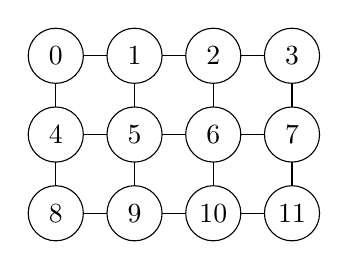
\begin{tikzpicture}
            \draw (0,0) grid (3,2);
            \foreach \x in {0,1,2,3} \foreach \y in {0,1,2}
                \draw (\x,\y) node[circle,draw,fill=white,inner sep=0,minimum size=0.7cm] {\pgfmathparse{int(8-4*\y+\x)}\pgfmathresult};
           \end{tikzpicture}
        \end{figure}
        \item[Delopgave 3 (30 point):] $2 \le N \le 100$.
        \item[Delopgave 4 (40 point):] $2 \le N \le 500$.
    \end{description}

    For at score maksimum point skal din løsning:
    \begin{enumerate}
    	\item Korrekt bestemme hvorvidt politibetjenten kan fange
   			  røveren.
   		\item Succesfuldt fange røveren ved at lave træk på
			  vegne af politibetjenten, hvis det er muligt.
    \end{enumerate}

    I delopgave 1 og 2 skal dit program implementere begge krav for at score
    nogen point. I delopgave 3 og 4 vil løsninger, der kun opfylder det første
	krav dog score 30\% af delopgavens point. Hvis dit program ikke opfylder
    det andet krav kan det i stedet afslutte sig selv ved at udføre et ulovligt
    træk (eksempelvis ved at returnere $-1$ i {\tt nextMove}).

    Bemærk at standardkravene (tids- og hukommelsesbegrænsning og ingen
    runtime errors) skal overholdes for at få nogen point.

    \Constraints

    \begin{description}
        \item[Tidsbegrænsning:] 1.5 s.
        \item[Hukommelsesbegrænsning:] 256 MB.
    \end{description}

    \Experimentation
    {\em Eksempel-graderen} på din computer kan læse data fra standard input
    som beskrevet herunder.
    Første linje af inputtet skal indeholde et heltal $N$ --- antallet af
    hjørner. De følgende $N$ linjer skal indeholde adjacency matricen $A$ (som
    beskrevet øverst side 2). Hver af disse linjer skal indeholde $N$ heltal,
    der hver er enten 0 eller 1. Matricen skal være symmetrisk og værdierne på
    diagonalen skal alle være nuller.

    Den næste linje skal indeholde 1, hvis politibetjenten kan fange røveren
    og 0 ellers.

    Endelig, hvis politibetjenten kan fange røveren, skal $N$ linjer følge,
    der beskriver røverens strategi. Hver af disse linjer skal indeholde
    $N+1$ heltal mellem $0$ og $N-1$. Værdien i række $r$ og søjle $c$,
    hvor $c < N$, svarer til en situation, hvor det er røverens tur,
    politibetjenten er på hjørne $r$ og røveren er på hjørne $c$, og værdien
    repræsenterer det hjørne, som røveren skal rykke til. Værdier på
    diagonalen vil blive ignoreret, da de svarer til situationer, hvor
    røveren og politibetjenten står på samme hjørne. Søjlen mest til højre
    definerer røverens starthjørner for hvert af politibetjentens mulige
    starthjørner.

    Her er et eksempel på input til eksempel-graderen, som repræsenterer tre
    hjørner, der alle er forbundet til hinanden:

    \begin{center}
        \begin{tabular}{p{4cm}}
            {\tt
                3 \newline
                0 1 1 \newline
                1 0 1 \newline
                1 1 0 \newline
                1 \newline
                0 2 1 2 \newline
                2 0 0 2 \newline
                1 0 0 1 \newline
            }
        \end{tabular}
    \end{center}

	Og her er input, der svarer til eksemplet givet i
	opgavebeskrivelsen:
    \begin{center}
        \begin{tabular}{p{4cm}}
            {\tt
                4 \newline
                0 1 1 1 \newline
                1 0 0 0 \newline
                1 0 0 0 \newline
                1 0 0 0 \newline
                1 \newline
                0 0 0 0 1 \newline
                2 0 0 0 2 \newline
                3 0 0 0 3 \newline
                1 0 0 0 1 \newline
            }
        \end{tabular}
    \end{center}
\end{document}
